\documentclass[a4paper,11pt,titlepage]{jarticle}
\usepackage[dvipdfmx]{graphicx}
\usepackage{listings}
\usepackage{amsmath}
\usepackage{fancybox,ascmac}

\title{アルゴリズムとデータ構造 : 第二回レポート}
\author{175751C 宮城孝明}
\date{\today}

\begin{document}
\maketitle
\tableofcontents
\clearpage

\section{課題}
選択法、挿入法、マージソート、クイックソートをプログラム化し処理時間を計測せよ。また計測結果を比較検討せよ。比較の際にはグラフを活用し効果的に行うこと。\par
\section{結果}
\begin{figure}[htbp]
  \centering
  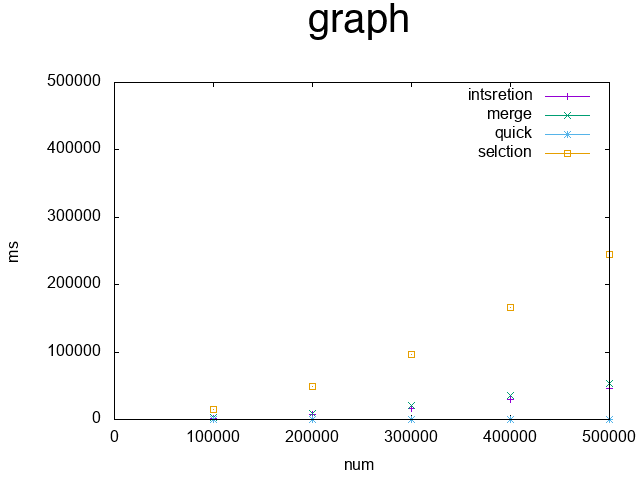
\includegraphics[width=100mm]{task1.png}
  \label{graph}
  \caption{アルゴリズムの計測時間の計測}
\end{figure}

\section{考察}
この結果を見て,Quicksortの速さがよくわかった。アルゴリズムが違うだけでここまでの処理にかかる時間が違う。そのため,同じ処理でもどちらでプログラムを組むのか慎重に考える必要がある。\par
\section{参考文献}
\begin{thebibliography}{}
  \bibitem{sibuta}sibat: a新・明解 Javaで学ぶアルゴリズムとデータ構造 (明解シリーズ) 
 \end{thebibliography}{}


\end{document} 
